\chapter{Summary and conclusion} %%%%%%%%%%%%%%%%%%%%%%%%%%%%%%%%%%%%%%%%%%%%%%%%%%%%%%%%%%%%%%%%%
\label{chap:conclusion} %%%%%%%%%%%%%%%%%%%%%%%%%%%%%%%%%%%%%%%%%%%%%%%%%%%%%%%%%%%%%%%%%%%%%%%%%%

- It is now abundantly clear that convolutional neural networks will play a key role in the event
reconstruction and classification for \chips. What is also clear is that other water Cherenkov
neutrino experiments, which up to now have not fully embraced modern machine learning techniques
as much as other sectors of the neutrino field should do so. For a range of benefits from
increased processing time, leverage the wider computer vision ML field to make the advancements
for you while you focus on the physics analysis.

% PERFORMANCE
\begin{enumerate}
    \item Sufficient cosmic rejection for negligible beam sample contamination is achieved.
    \item Beam classification selection is surprisingly comparable to other costly experiments.
    \item Energy estimation is comparable and more generalisable compared to standard methods.
    \item Cherenkov ring and Hough peak features are clearly being learnt by the trained networks.
    \item There is clear learnt separation between categories as seen via unsupervised methods.
    \item Future work should train beam classification network on only contained events.
    \item The smearing of hit times is found to have a negligible impact on performance.
    \item Robust to charge calibration.
    \item Random PMT noise is found to have a negligible impact on performance.
    \item The input representation of the event is important for performance.
    \item The training sample must match the expected composition of events closely.
    \item The network architecture does not matter much in the context of this work.
    \item Future work should explore larger input image sizes and network architectures.
    \item Future work should study the input distribution of events in greater detail.
    \item Future work should look at using a graph convolutional network or transformers.
\end{enumerate}

\begin{figure} % CHIPS RAMP DIAGRAM %
    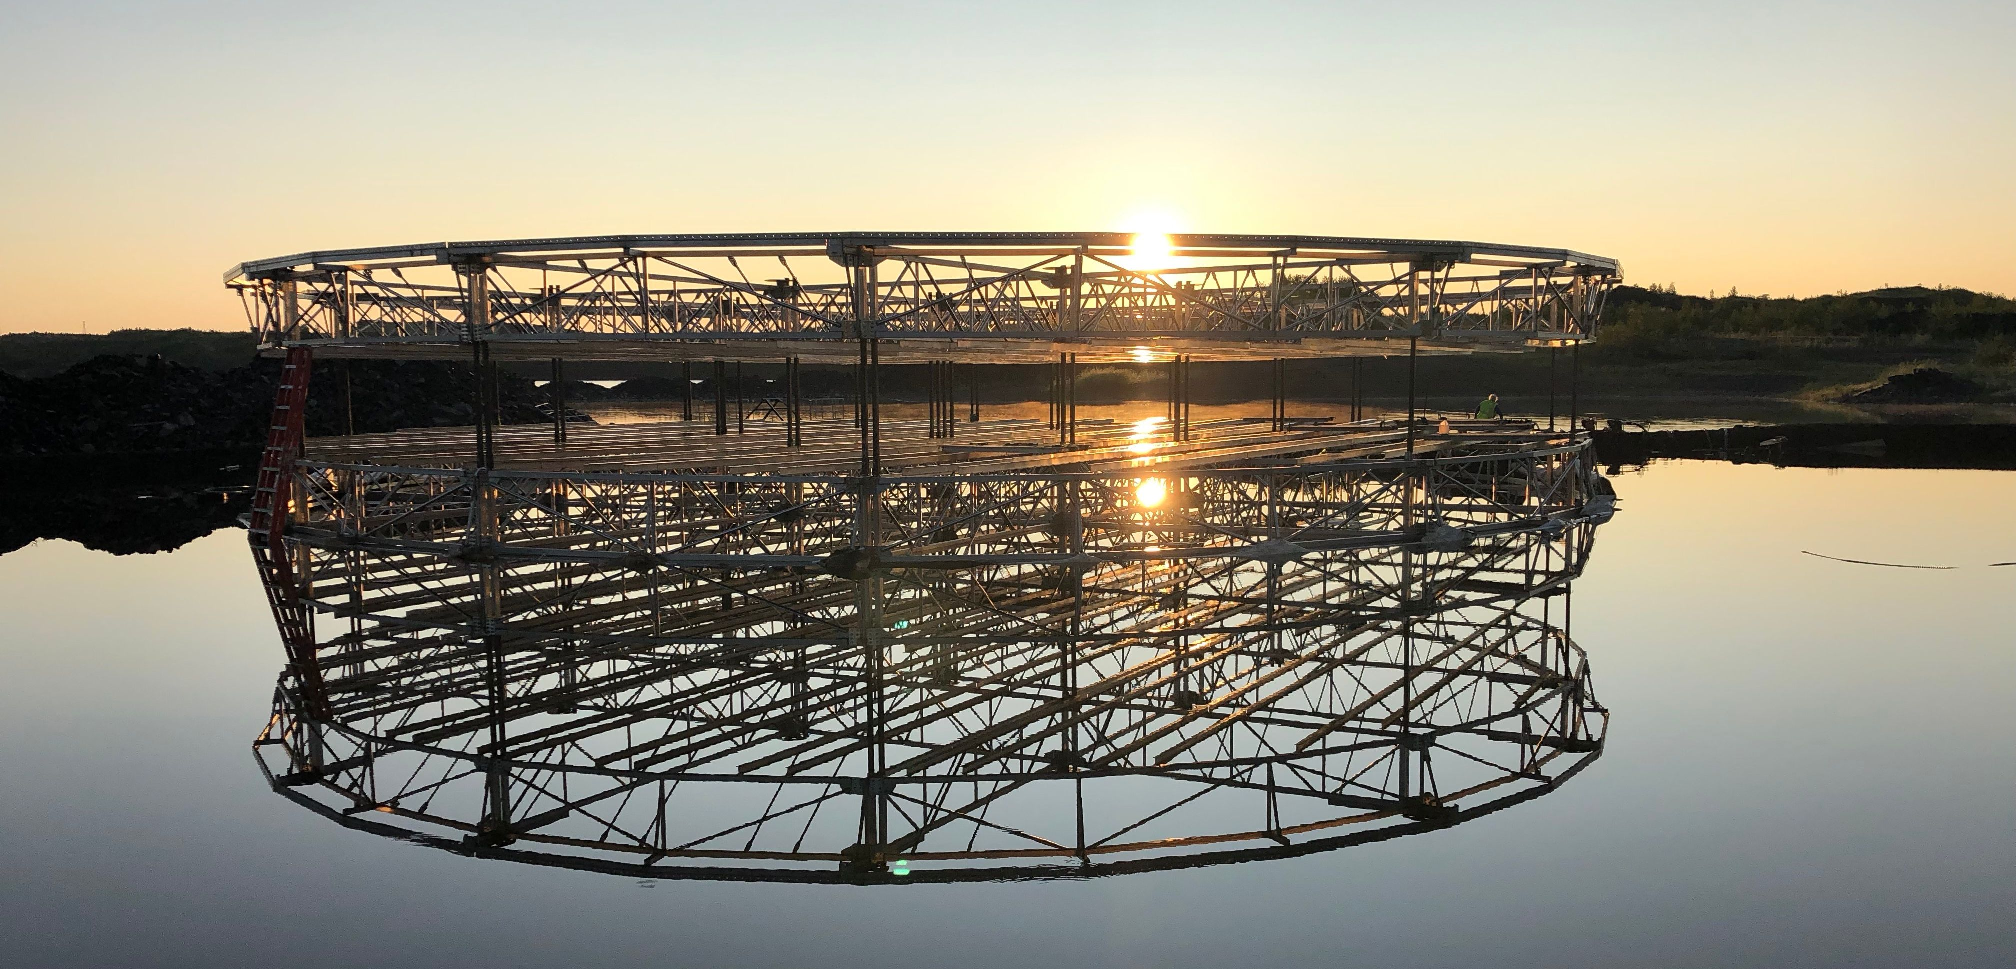
\includegraphics[width=\textwidth]{diagrams/4-chips/sunrise.pdf}
    \caption*{The \chipsfive detector frame at sunrise.}
\end{figure}

- Turns out neutrino water Cherenkov detectors produce as output an image-like event suitable for
modern Computer Vision techniques using Convolutional Neural Networks, a type of deep learning.

- Allowing for vastly increased speed with which analysis can be conducted and less reliance on
heavily human influenced bespoke software frameworks.

- This is fundamentally the primary event analysis task for water Cherenkov neutrino detectors.
Neutrino interactions within the detector create rings of light that are recorded on the walls of
the detector, these are used to infer the properties on the underlying neutrino interaction.